


\tikzset{every picture/.style={line width=0.75pt}} %set default line width to 0.75pt       
\begin{figure}[htbp]
\centering


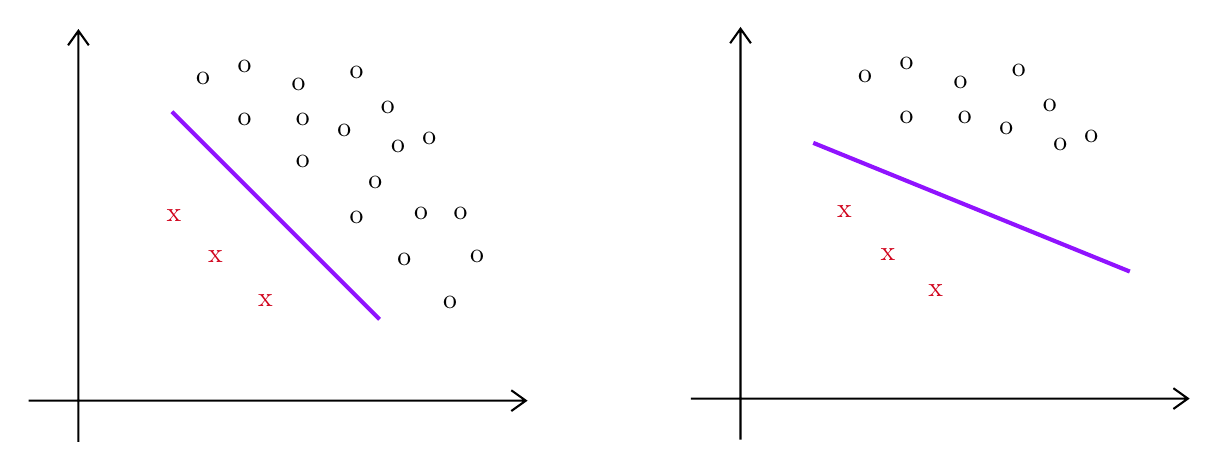
\begin{tikzpicture}[x=0.75pt,y=0.75pt,yscale=-1,xscale=1]
%uncomment if require: \path (0,300); %set diagram left start at 0, and has height of 300

%Shape: Axis 2D [id:dp33720031646484827] 
\draw  (50,215.2) -- (289.5,215.2)(73.95,37) -- (73.95,235) (282.5,210.2) -- (289.5,215.2) -- (282.5,220.2) (68.95,44) -- (73.95,37) -- (78.95,44)  ;
%Straight Lines [id:da49156386348114545] 
\draw [color={rgb, 255:red, 144; green, 19; blue, 254 }  ,draw opacity=1 ][fill={rgb, 255:red, 144; green, 19; blue, 254 }  ,fill opacity=1 ][line width=1.5]    (119,76) -- (219,176) ;


%Shape: Axis 2D [id:dp9978017465833935] 
\draw  (369,214.2) -- (608.5,214.2)(392.95,36) -- (392.95,234) (601.5,209.2) -- (608.5,214.2) -- (601.5,219.2) (387.95,43) -- (392.95,36) -- (397.95,43)  ;
%Straight Lines [id:da6705581541742359] 
\draw [color={rgb, 255:red, 144; green, 19; blue, 254 }  ,draw opacity=1 ][fill={rgb, 255:red, 144; green, 19; blue, 254 }  ,fill opacity=1 ][line width=1.5]    (428,91) -- (580.5,153) ;



% Text Node
\draw (134,60) node  [align=left] {o};
% Text Node
\draw (154,80) node  [align=left] {o};
% Text Node
\draw (182,100) node  [align=left] {o};
% Text Node
\draw (180,63) node  [align=left] {o};
% Text Node
\draw (202,85) node  [align=left] {o};
% Text Node
\draw (217,110) node  [align=left] {o};
% Text Node
\draw (208,127) node  [align=left] {o};
% Text Node
\draw (231,147) node  [align=left] {o};
% Text Node
\draw (258,125) node  [align=left] {o};
% Text Node
\draw (253,168) node  [align=left] {o};
% Text Node
\draw (243,89) node  [align=left] {o};
% Text Node
\draw (208,57) node  [align=left] {o};
% Text Node
\draw (154,54) node  [align=left] {o};
% Text Node
\draw (182,80) node  [align=left] {o};
% Text Node
\draw (223,74) node  [align=left] {o};
% Text Node
\draw (239,125) node  [align=left] {o};
% Text Node
\draw (266,146) node  [align=left] {o};
% Text Node
\draw (228,93) node  [align=left] {o};
% Text Node
\draw (120,126) node [color={rgb, 255:red, 208; green, 2; blue, 27 }  ,opacity=1 ] [align=left] {x};
% Text Node
\draw (140,146) node [color={rgb, 255:red, 208; green, 2; blue, 27 }  ,opacity=1 ] [align=left] {x};
% Text Node
\draw (164,167) node [color={rgb, 255:red, 208; green, 2; blue, 27 }  ,opacity=1 ] [align=left] {x};
% Text Node
\draw (453,59) node  [align=left] {o};
% Text Node
\draw (473,79) node  [align=left] {o};
% Text Node
\draw (499,62) node  [align=left] {o};
% Text Node
\draw (521,84) node  [align=left] {o};
% Text Node
\draw (562,88) node  [align=left] {o};
% Text Node
\draw (527,56) node  [align=left] {o};
% Text Node
\draw (473,53) node  [align=left] {o};
% Text Node
\draw (501,79) node  [align=left] {o};
% Text Node
\draw (542,73) node  [align=left] {o};
% Text Node
\draw (547,92) node  [align=left] {o};
% Text Node
\draw (443,124) node [color={rgb, 255:red, 208; green, 2; blue, 27 }  ,opacity=1 ] [align=left] {x};
% Text Node
\draw (464,145) node [color={rgb, 255:red, 208; green, 2; blue, 27 }  ,opacity=1 ] [align=left] {x};
% Text Node
\draw (487,162) node [color={rgb, 255:red, 208; green, 2; blue, 27 }  ,opacity=1 ] [align=left] {x};


\end{tikzpicture}

\caption{Undersampling} \label{fig:Undersampling}
\end{figure}